
\pagebreak
\section{Shapley Value Approximation}\label{sec:shapley}

The Shapley value is a cornerstone measure in cooperative game theory. 
It is an axiomatic approach to allocating a divisible reward or cost between participants where there is a clearly defined notion of how much surplus or profit a group or ``coalition'' of participants could achieve by themselves \citep{ChalkiadakisEtAl2012}.
It has many applications, 
including analyzing the power of voting blocks in weighted voting games \citep{Bachrach2009ApproximatingPI}, 
in cost and surplus division problems  \citep{AzizEtal2016,archie_paper1}, 
and as a measure of network centrality \citep{Michalak:2013}.

Formally, a \textit{cooperative game}, $\langle N,v\rangle\in\mathbb{G}_N$, comprises a set of $n$ players, $N=\{1,2,\dots,n\}$, and a \textit{characteristic function}, $v:S\subset N\rightarrow \mathbb{R}$, which is a function specifying the reward which can be achieved if a subset of the players $S\subset N$ cooperate, where $v(\emptyset)=0$.
In this context the Shapley value $\varphi$ is a unique mapping from cooperative games to the player rewards $\mathbb{G}_N\rightarrow\mathbb{R}^n$ which satisfies axioms:

\begin{itemize}
\item	
\textbf{Efficiency}: That the total reward is divided up: $\sum_i\varphi_i(\langle N,v\rangle) = v(N)$
\item	
\textbf{Symmetry}: If two players $i$ and $j$ are totally equivalent `substitutes' then the receive the same reward: ie. if $v(S\cup i)=v(S\cup j)~~\forall S\subseteq N\setminus\{i,j\}$, then $\varphi_i(\langle N,v\rangle) = \varphi_i(\langle N,v\rangle)$
\item	
\textbf{Null Player}: If the addition of a player $i$ to any coalition brings nothing, and is a `null player', then it receives reward of zero: i.e if $v(S\cup i)=v(S)~~\forall S\subseteq N$ then $\varphi_i(\langle N,v\rangle)=0$
\item	
\textbf{Additivity}: That for any two games the reward afforded each player is each is the sum of the games considered together: i.e. for any $v_1$ and $v_2$, that: $\varphi(\langle N,v_1+v_2\rangle)=\varphi(\langle N,v_1 \rangle) + \varphi(\langle N,v_2\rangle)$
\end{itemize}

Specifically, the Shapley value is expressed as:
\begin{equation}\label{shap1}\varphi_i(\langle N,v\rangle) = \sum_{S\subset N, i\notin S}\frac{(n-|S|-1)!\,|S|!}{n!}(v(S\cup\{i\})-v(S))\end{equation}
That is, under the Shapley value each player is afforded their average marginal contribution across every possible sequence of player join orderings.  
Or, if $v_{i,k}$ is the average marginal contribution which player $i$ can make across coalitions of size $k$:
\begin{equation}
v_{i,k} = \frac{1}{\binom{n-1}{k}}\sum_{S\subset N\setminus \{ i\} , |S|=k} %\frac{(n-|S|-1)!\,|S|!}{(n-1)!}
(v(S\cup\{i\})-v(S))
\end{equation}
then the Shapley value can be expressed as an average:
\begin{equation}\label{shap2} \varphi_i(\langle N,v\rangle) = \frac{1}{n}\sum_{k=0}^{n-1}v_{i,k} \end{equation}
Though the Shapley value is conceptually simple, its use is hampered by the fact that its total expression involves exponentially many evaluations of the characteristic function (there are $n\times 2^{n-1}$ possible marginal contributions between $n$ players).

However, since the Shapley value is expressible as an average over averages by Equation~\eqref{shap2}, 
it is possible to approximate these averages via sampling techniques, and these averages are naturally stratified by coalition size.
In previously published literature, other techniques have been used to allocate samples in this context, particularly simple sampling \citep{DBLP:journals/cor/CastroGT09}, Neyman allocation \citep{CASTRO2017180,DBLP:journals/tsg/OBrienGR15}, and allocation to minimize Hoeffding's inequality \citep{2013arXiv1306.4265M}.

We assess the benefits of using our bound by comparing its performance to the approaches above in the context of some example cooperative games, with results analyzed in Section~\ref{sec:discussion}.
The example games are described below:

\begin{example_game}[Airport Game]
An $n=15$ player game with characteristic function:
$$v(S)=\max_{i\in S}w_i$$
where
$w=\{w_1,\dots,w_{15}\} %\scriptstyle\scriptsize
=\{ 1, 1, 2, 2, 2, 3, 4, 5, 5, 5, 7, 8, 8, 8, 10\}$.
The maximum marginal contribution is $10$, so we assign $D_i=10$ for all $i$.
\end{example_game}

\begin{example_game}[Voting Game]
An $n=15$ player game with characteristic function:
$$v(S)=\begin{cases}
       1, &\quad\text{if}\quad \sum_{i\in S}w_i>\sum_{j\in N}w_j/2\\
       0, &\quad\text{otherwise}\\
     \end{cases}$$
where 
$w=\{w_1,\dots,w_{15}\} %\scriptstyle\scriptsize
=\{ 1, 3, 3, 6, 12, 16, 17, 19, 19, 19, 21, 22, 23, 24, 29\}$.
The maximum marginal contribution is $1$, so we assign $D_i=1$ for all $i$.
\end{example_game}

\begin{example_game}[Simple Reward Division]
An $n=15$ player game with characteristic function:
$$v(S)=\frac{1}{2}\left(\sum_{i\in S}\frac{w_i}{100}\right)^2$$
where
$w=\{w_1,\dots,w_{15}\} = \{ 45, 41, 27, 26, 25, 21, 13, 13, 12, 12, 11, 11, 10, 10, 10 \}$\\
The maximum marginal contribution is $1.19025$, so we assign $D_i=1.19025$ for all $i$.
\end{example_game}

\begin{example_game}[Complex Reward Division]
An $n=15$ player game with characteristic function:
$$v(S)=\left(\sum_{i\in S}\frac{w_i}{50}\right)^2 - \floor[\Bigg]{\sum_{i\in S}\frac{w_i}{50}}^2$$
where
$w=\{w_1,\dots,w_{15}\} = \{ 45, 41, 27, 26, 25, 21, 13, 13, 12, 12, 11, 11, 10, 10, 10 \}$\\
In this game, we assign $D_i=2$ for all $i$.
\end{example_game}

%\input{table-2.tex}





\begin{table*}[]
    \centering 
    \begin{minipage}[]{0.8\textwidth}
        \centering
        \caption{Airport Game Average Errors}\label{tab1}
			\begin{tabular}{llllll}
			\hline
			$\nicefrac{m}{n^2}$ & $10$ & $50$ & $100$ & $500$ & $1000$ \\
			\hline
			$e^{Ma}$   & 298.4 & 133.1 & 99.64 & 41.96 & 29.26 \\
			$e^{sim}$  & 357.8 & 146.1 & 106.2 & 44.55 & 36.33 \\
			$e^{Ca}$   & 325.7 & 115.8 & 75.85 & 31.01 & 22.12 \\
			$e^{SEBM}$ & 259.2 & 73.8 & 54.76 & 7.71 & 1.30  \\
			\hline
			\end{tabular}
    \end{minipage}
	\\\vspace{4mm}
    \begin{minipage}[]{0.8\textwidth}
        \centering
        \caption{Voting Game Average Errors}\label{tab2}
			\begin{tabular}{llllll}
			\hline
			$\nicefrac{m}{n^2}$ & $10$ & $50$ & $100$ & $500$ & $1000$ \\
			\hline
			$e^{Ma}$    & 131.0 & 57.78 & 41.52 & 18.66 & 13.18 \\
			$e^{sim}$   & 145.7 & 59.72 & 40.31 & 17.56 & 12.84 \\
			$e^{Ca}$    & 142.1 & 47.35 & 31.05 & 14.08 & 9.800 \\
			$e^{SEBM}$  & 122.8 & 47.44 & 33.18 & 8.55 & 1.995  \\
			\hline
			\end{tabular}
    \end{minipage}
	\\\vspace{4mm}
    \begin{minipage}[]{0.8\textwidth}
        \centering
        \caption{Simple Reward Division Game average errors}\label{tab3}
			\begin{tabular}{llllll}
			\hline
			$\nicefrac{m}{n^2}$ & $10$ & $50$ & $100$ & $500$ & $1000$ \\
			\hline
			$e^{Ma}$    & 25.68 & 11.62 & 7.792 & 3.481 & 2.290 \\
			$e^{sim}$   & 22.10 & 9.045 & 6.218 & 2.642 & 1.938 \\
			$e^{Ca}$    & 22.37 & 8.925 & 6.692 & 2.727 & 1.940 \\
			$e^{SEBM}$  & 19.25 & 7.044 & 5.158 & 1.183 & 0.2817  \\
			\hline
			\end{tabular}
    \end{minipage}
	\\\vspace{4mm}
    \begin{minipage}[]{0.8\textwidth}
        \centering
        \caption{Complex Reward Division Game average errors}\label{tab4}
			\centering
			\begin{tabular}{llllll}
			\hline
			$\nicefrac{m}{n^2}$ & $10$ & $50$ & $100$ & $500$ & $1000$ \\
			\hline
			$e^{Ma}$   & 276.1 & 118.9 & 87.00 & 40.15 & 27.44 \\
			$e^{sim}$  & 251.4 & 108.0 & 78.63 & 34.64 & 26.82 \\
			$e^{Ca}$   & 290.5 & 116.5 & 81.82 & 35.70 & 26.50 \\
			$e^{SEBM}$ & 214.2 & 78.47 & 54.10 & 12.45 & 2.711  \\
			\hline
			\end{tabular}
    \end{minipage}
    \vspace{3mm}
    \caption{Average absolute errors in the Shapley value calculation across all players in the four cooperative games (units in $10^{-4}$), for the different sampling schemes with different sampling budgets $m$ per number of strata (with $n^2=15^2$ for all).}
    \label{Table2}
\end{table*}



For each game, we compute the exact Shapley value, and then the average absolute errors in the approximated Shapley value for a given budget $m$ of marginal-contribution samples across multiple computational runs.
The results are shown in Table \ref{Table2}, 
where the average absolute error in the Shapley value is computed by sampling with Maleki's method \citep{2013arXiv1306.4265M} is denoted $e^{Ma}$, $e^{sim}$ is Castro's stratified simple sampling method \citep{DBLP:journals/cor/CastroGT09}, $e^{Ca}$ is Castro's Neyman sampling method \citep{CASTRO2017180}, and $e^{SEBM}$ is the error associated with our method, SEBM. 
The results in Table~\ref{Table2} show that our method performs well across the benchmarks. 
A discussion of all of the results is considered in the next section. 


\section{Discussion}
\label{sec:discussion}

In this section we give considerations to the numerical results of this chapter.
In general, from the results across Figures~\ref{Table1},\ref{Table111} and \ref{biggraph3} and Table \ref{Table2}, the main observation is that most of the techniques performed well and similar to Neyman sampling, and that our sampling technique, SEBM (or SEBM-W) and SECM performed competitively to Neyman sampling (\textsc{Ney} or \textsc{Ney-W}) despite not having access to knowledge of strata variances.
It is also observed that Neyman sampling was ultimately the most accurate, for reasons allready presented in section \ref{sec:neyman_sampling}.
Particularly that if sufficient samples have been taken then the sample means of the strata will tend to approximately be Gaussian distributed by the Central Limit Theorem.
In this context the strata means have a distribution that is entirely characterised by their mean and variance, and hence so too therefore is the population mean estimate.
Hence the variance of the sampled population mean is the only parameter controlling the error, and minimising it directly translates into improved accuracy.

One of the most remarkable inferences from the data is just how very readily Central Limit Theorem dynamics emerges, from Figure \ref{fig:central_limit_theorem} we can see that the sample error of uniformly distributed data converges almost perfectly to a gaussian distribution even in just 4 samples.


    \begin{figure}[]
        \centering
		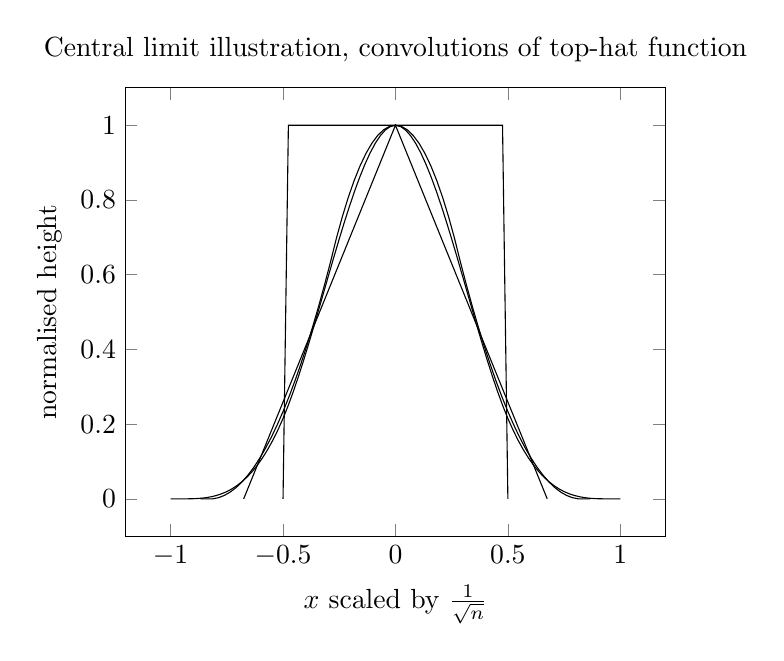
\begin{tikzpicture}
		\begin{axis}[
			title={Central limit illustration, convolutions of top-hat function},
			xlabel={$x$ scaled by $\frac{1}{\sqrt{n}}$},
			ylabel={normalised height},
		]
		\addplot[black] coordinates {
(-0.5, 0.0)(-0.47619047619047616, 1.0)(-0.4523809523809524, 1.0)(-0.4285714285714286, 1.0)(-0.40476190476190477, 1.0)(-0.38095238095238093, 1.0)(-0.35714285714285715, 1.0)(-0.33333333333333337, 1.0)(-0.30952380952380953, 1.0)(-0.2857142857142857, 1.0)(-0.2619047619047619, 1.0)(-0.23809523809523808, 1.0)(-0.2142857142857143, 1.0)(-0.19047619047619047, 1.0)(-0.16666666666666669, 1.0)(-0.14285714285714285, 1.0)(-0.11904761904761907, 1.0)(-0.09523809523809523, 1.0)(-0.07142857142857145, 1.0)(-0.047619047619047616, 1.0)(-0.023809523809523836, 1.0)(0.0, 1.0)(0.023809523809523836, 1.0)(0.04761904761904767, 1.0)(0.0714285714285714, 1.0)(0.09523809523809523, 1.0)(0.11904761904761907, 1.0)(0.1428571428571429, 1.0)(0.16666666666666663, 1.0)(0.19047619047619047, 1.0)(0.2142857142857143, 1.0)(0.23809523809523814, 1.0)(0.26190476190476186, 1.0)(0.2857142857142857, 1.0)(0.30952380952380953, 1.0)(0.33333333333333337, 1.0)(0.3571428571428571, 1.0)(0.38095238095238093, 1.0)(0.40476190476190477, 1.0)(0.4285714285714286, 1.0)(0.45238095238095233, 1.0)(0.47619047619047616, 1.0)(0.5, 0.0)
        }node[pos=0.91](endofplotsquare){} ;
		%\node [below,color={rgb:red,0;green,0;yellow,0}] at (endofplotsquare) {\footnotesize Our Bound};
		\addplot[black] coordinates {
(-0.6749655638598864, 0.0)(-0.6428243465332251, 0.047619047619047616)(-0.6106831292065639, 0.09523809523809523)(-0.5785419118799026, 0.14285714285714285)(-0.5464006945532413, 0.19047619047619047)(-0.51425947722658, 0.23809523809523808)(-0.48211825989991886, 0.2857142857142857)(-0.44997704257325755, 0.3333333333333333)(-0.41783582524659624, 0.38095238095238093)(-0.385694607919935, 0.42857142857142855)(-0.3535533905932738, 0.47619047619047616)(-0.3214121732666126, 0.5238095238095238)(-0.2892709559399513, 0.5714285714285714)(-0.25712973861329, 0.6190476190476191)(-0.2249885212866288, 0.6666666666666666)(-0.1928473039599675, 0.7142857142857143)(-0.1607060866333063, 0.7619047619047619)(-0.12856486930664499, 0.8095238095238095)(-0.09642365197998375, 0.8571428571428571)(-0.06428243465332253, 0.9047619047619048)(-0.032141217326661226, 0.9523809523809523)(0.0, 1.0)(0.032141217326661226, 0.9523809523809523)(0.06428243465332245, 0.9047619047619048)(0.09642365197998383, 0.8571428571428571)(0.12856486930664507, 0.8095238095238095)(0.1607060866333063, 0.7619047619047619)(0.1928473039599675, 0.7142857142857143)(0.22498852128662872, 0.6666666666666666)(0.25712973861328997, 0.6190476190476191)(0.28927095593995134, 0.5714285714285714)(0.3214121732666126, 0.5238095238095238)(0.3535533905932738, 0.47619047619047616)(0.385694607919935, 0.42857142857142855)(0.41783582524659624, 0.38095238095238093)(0.4499770425732576, 0.3333333333333333)(0.48211825989991886, 0.2857142857142857)(0.51425947722658, 0.23809523809523808)(0.5464006945532413, 0.19047619047619047)(0.5785419118799026, 0.14285714285714285)(0.6106831292065638, 0.09523809523809523)(0.6428243465332252, 0.047619047619047616)(0.6749655638598864, 0.0)
        }node[pos=0.5](endofplotsquare){} ;
		%\node [above,color={rgb:red,0;blue,0;yellow,0}, rotate=-45] at (endofplotsquare) {\footnotesize Entropy};
		\addplot[black] coordinates {
(-0.8660254037844386, 0.0)(-0.8397822097303648, 0.0)(-0.8135390156762908, 0.0)(-0.7872958216222169, 0.0030211480362537764)(-0.761052627568143, 0.00906344410876133)(-0.7348094335140691, 0.01812688821752266)(-0.7085662394599952, 0.030211480362537766)(-0.6823230454059213, 0.045317220543806644)(-0.6560798513518474, 0.0634441087613293)(-0.6298366572977735, 0.08459214501510574)(-0.6035934632436997, 0.10876132930513595)(-0.5773502691896258, 0.13595166163141995)(-0.5511070751355518, 0.1661631419939577)(-0.524863881081478, 0.19939577039274925)(-0.498620687027404, 0.23564954682779457)(-0.4723774929733301, 0.27492447129909364)(-0.4461342989192562, 0.31722054380664655)(-0.4198911048651824, 0.36253776435045315)(-0.3936479108111085, 0.4108761329305136)(-0.3674047167570345, 0.4622356495468278)(-0.34116152270296063, 0.5166163141993958)(-0.31491832864888675, 0.5740181268882175)(-0.2886751345948129, 0.6344410876132931)(-0.26243194054073893, 0.6978851963746223)(-0.23618874648666505, 0.7552870090634441)(-0.2099455524325912, 0.8066465256797583)(-0.1837023583785173, 0.851963746223565)(-0.15745916432444335, 0.8912386706948641)(-0.13121597027036946, 0.9244712990936556)(-0.1049727762162956, 0.9516616314199395)(-0.07872958216222171, 0.972809667673716)(-0.05248638810814775, 0.9879154078549849)(-0.026243194054073875, 0.9969788519637462)(0.0, 1.0)(0.026243194054073875, 0.9969788519637462)(0.05248638810814775, 0.9879154078549849)(0.07872958216222162, 0.972809667673716)(0.1049727762162955, 0.9516616314199395)(0.13121597027036955, 0.9244712990936556)(0.15745916432444343, 0.8912386706948641)(0.1837023583785173, 0.851963746223565)(0.2099455524325912, 0.8066465256797583)(0.23618874648666505, 0.7552870090634441)(0.26243194054073893, 0.6978851963746223)(0.2886751345948128, 0.6344410876132931)(0.3149183286488867, 0.5740181268882175)(0.34116152270296074, 0.5166163141993958)(0.3674047167570346, 0.4622356495468278)(0.3936479108111085, 0.4108761329305136)(0.4198911048651824, 0.36253776435045315)(0.4461342989192562, 0.31722054380664655)(0.4723774929733301, 0.27492447129909364)(0.498620687027404, 0.23564954682779457)(0.5248638810814779, 0.19939577039274925)(0.5511070751355519, 0.1661631419939577)(0.5773502691896258, 0.13595166163141995)(0.6035934632436997, 0.10876132930513595)(0.6298366572977735, 0.08459214501510574)(0.6560798513518474, 0.0634441087613293)(0.6823230454059213, 0.045317220543806644)(0.7085662394599952, 0.030211480362537766)(0.734809433514069, 0.01812688821752266)(0.7610526275681431, 0.00906344410876133)(0.787295821622217, 0.0030211480362537764)(0.8135390156762908, 0.0)(0.8397822097303648, 0.0)(0.8660254037844386, 0.0)
        }node[pos=0.7](endofplotsquare){} ;
		%\node [below,black, rotate=-45] at (endofplotsquare) {\footnotesize Efron};
		\addplot[black] coordinates {
(-1.0, 0.0)(-0.9772727272727273, 0.0)(-0.9545454545454546, 0.0)(-0.9318181818181819, 0.0)(-0.9090909090909091, 0.00016178611875101117)(-0.8863636363636364, 0.0006471444750040447)(-0.8636363636363636, 0.0016178611875101116)(-0.8409090909090909, 0.003235722375020223)(-0.8181818181818181, 0.0056625141562853904)(-0.7954545454545454, 0.009060022650056626)(-0.7727272727272727, 0.013590033975084938)(-0.75, 0.01941433425012134)(-0.7272727272727273, 0.026694709593916843)(-0.7045454545454546, 0.03559294612522246)(-0.6818181818181819, 0.046270829962789195)(-0.6590909090909092, 0.05889014722536806)(-0.6363636363636364, 0.07361268403171008)(-0.6136363636363636, 0.09060022650056625)(-0.5909090909090908, 0.11001456075068759)(-0.5681818181818181, 0.1320174729008251)(-0.5454545454545454, 0.15677074906972982)(-0.5227272727272727, 0.18443617537615273)(-0.5, 0.21517553793884484)(-0.4772727272727273, 0.2491506228765572)(-0.4545454545454546, 0.2865232163080408)(-0.43181818181818177, 0.32680795987704253)(-0.40909090909090906, 0.3695194952273095)(-0.38636363636363635, 0.41417246400258856)(-0.36363636363636365, 0.46028150784662675)(-0.34090909090909094, 0.507361268403171)(-0.31818181818181823, 0.5549263873159683)(-0.2954545454545454, 0.6024915062287656)(-0.2727272727272727, 0.6495712667853099)(-0.25, 0.695680310629348)(-0.2272727272727273, 0.7403332794046271)(-0.20454545454545459, 0.7830448147548941)(-0.18181818181818177, 0.8233295583238958)(-0.15909090909090906, 0.8607021517553793)(-0.13636363636363635, 0.8946772366930917)(-0.11363636363636365, 0.9247694547807798)(-0.09090909090909094, 0.9504934476621906)(-0.06818181818181823, 0.971363856981071)(-0.045454545454545414, 0.9868953243811681)(-0.022727272727272707, 0.9966024915062288)(0.0, 1.0)(0.022727272727272707, 0.9966024915062288)(0.045454545454545414, 0.9868953243811681)(0.06818181818181812, 0.971363856981071)(0.09090909090909083, 0.9504934476621906)(0.11363636363636354, 0.9247694547807798)(0.13636363636363646, 0.8946772366930917)(0.15909090909090917, 0.8607021517553793)(0.18181818181818188, 0.8233295583238958)(0.20454545454545459, 0.7830448147548941)(0.2272727272727273, 0.7403332794046271)(0.25, 0.695680310629348)(0.2727272727272727, 0.6495712667853099)(0.2954545454545454, 0.6024915062287656)(0.3181818181818181, 0.5549263873159683)(0.34090909090909083, 0.507361268403171)(0.36363636363636354, 0.46028150784662675)(0.38636363636363646, 0.41417246400258856)(0.40909090909090917, 0.3695194952273095)(0.4318181818181819, 0.32680795987704253)(0.4545454545454546, 0.2865232163080408)(0.4772727272727273, 0.2491506228765572)(0.5, 0.21517553793884484)(0.5227272727272727, 0.18443617537615273)(0.5454545454545454, 0.15677074906972982)(0.5681818181818181, 0.1320174729008251)(0.5909090909090908, 0.11001456075068759)(0.6136363636363635, 0.09060022650056625)(0.6363636363636365, 0.07361268403171008)(0.6590909090909092, 0.05889014722536806)(0.6818181818181819, 0.046270829962789195)(0.7045454545454546, 0.03559294612522246)(0.7272727272727273, 0.026694709593916843)(0.75, 0.01941433425012134)(0.7727272727272727, 0.013590033975084938)(0.7954545454545454, 0.009060022650056626)(0.8181818181818181, 0.0056625141562853904)(0.8409090909090908, 0.003235722375020223)(0.8636363636363635, 0.0016178611875101116)(0.8863636363636365, 0.0006471444750040447)(0.9090909090909092, 0.00016178611875101117)(0.9318181818181819, 0.0)(0.9545454545454546, 0.0)(0.9772727272727273, 0.0)(1.0, 0.0)
        }node[pos=0.7](endofplotsquare){} ;
		%\node [below,black, rotate=-45] at (endofplotsquare) {\footnotesize Efron};
		
		\end{axis}
		\end{tikzpicture}
		%\vspace{-18pt}
		\caption[Self convolutions of the top hat function]{self convolutions of the top hat function (ie. probability distribution of the uniform function) for $n=1,2,3,4$ shows rapid convergence to gaussian distribution}
		\label{fig:central_limit_theorem}
    \end{figure}


This dynamic speaks strongly to the efficiency of Neyman sampling, and indeed our method SEBM* performs worse as it extends from minimising a simplification of Bennett's inequality - this is most evident in figure \ref{biggraph3}.\footnote{we would expect that a method consisting of minimising Bennett's inequality proper, would yeild extremely similar results to Neyman sampling}.
One of the more interesting things is the relative inefficiency of the SECM method, particularly as it sought to minimise Chebyshev's inequality for the stratified sampling, and under perfect variance information would be identical to Neyman sampling.
The implication about this context is that the inefficiency of utilising these methods primarily extends from uncertainty about the variances of the strata.
The Bernoulli-uniform data results (plotted in \ref{biggraph3}) were specifically designed to amplify the detriment in stratified sampling that uncertainty about the variances would yeild.
And that the more infrequent the bernoulli outlier, the more likely that the methods without variance information would over-sample the bernoulli stratum - which they did.
It is interesting that the SEBM* method also did this to some extent, although it is not particularly clear exactly why.


From between Figures~\ref{Table1} and \ref{Table111} we observe that sampling without replacement always performs better than sampling with replacement for the same method. 
This improvement is magnified as the number of samples grows large relative to the size of the population. 
At the same time, simple \textsc{Random} sampling almost always performs worst, because it fails to take advantage of any variance information. and \textsc{Simple} sampling performs even worse as it fails to take into account data stratification, These results are as expected.
From the Figures ~\ref{Table1} and \ref{Table111} we see that the primary increase in performance comes from employing stratified sampling over simple sampling, sampling without replacement over sampling with replacement, and then using some method that is more intellegent than randomly selecting samples and preferrably using stratum variance information to get close to the ideal of Neyman sampling.

%Next, note that the results of Figure~\ref{Table1} show that there is a mid-range of sample sizes where choosing a different method can even have a greater impact on sampling efficiency and rate of average error reduction than the difference between sampling with or without replacement.
%This is an important insight, as sampling real-world data (e.g. surveys, polling, destructive testing, etc) can be an expensive and slow process.
%Accordingly an appropriate method of choosing numbers of samples can lead to a material difference in cost for the same accuracy.
%There is also a slight decrease in the performance of SEBM* in comparison with \textsc{Ney} in the case of high number of samples and sampling without replacement, as illustrated in Figure~\ref{Table1}. 
%This indicates that the use of sub-optimal equation~\ref{approx1} in the derivation of Lemma~\ref{martingale0} might have some negative effect, by distorting the shape of the functions that the sampling processes then minimizes.

%If the data features very rare events, then SEBM and SEBM* seem to perform in a manner less than ideal.
%These condition are illustrated in Figure~\ref{biggraph3}, where the more rare the Bernoulli variable successes, the worse our methods perform in comparison with Neyman sampling (\textsc{Ney}).
%This shortcoming can be partly explained by noting that SEBM unnecessarily wastes samples on the Bernoulli stratum of rare events in the process of learning that the variance is almost zero, whereas \textsc{Ney} can avoid this because it has prior knowledge of the variances to begin with. 
%As such, this factor explains the difference between the performance of SEBM and SEBM* in the context of Figure~\ref{Table1} and also in Figure~\ref{biggraph3}.
%What is surprising is how small the difference in performance between SEBM and SEBM* is. 
%This indicates that as additional samples are taken, the original uncertainty about the strata variances have less and less effect upon the total numbers of samples that are eventually drawn from each of the strata.

%However, the performance difference between SEBM* and \textsc{Ney} in Figure~\ref{biggraph3} is not explained by this argument, as they use the same information.
%Instead, the reason for this difference in performance is found by considering the simplifying approximation of Equation \eqref{eq:part2} in the derivation of Lemma~\ref{expectation1}. 
%Specifically, \eqref{eq:part2} introduces a particular distortion into the shape of Equation~\eqref{big_equation} which our sampling seeks to minimize.
%Figure~\ref{fig:graph2} illustrates how the approximation \eqref{eq:part2} loosens the bound with respect to the variance. 
%Observe that when the variances are very small that Equation~\eqref{eq:part3} overly loosens the bounds, causing oversampling of strata with very small variances. 
%It appears that this factor is at play in the under-performance shown in Figure~\ref{biggraph3} and also the slight under-performance of our method in the Voting Game in Table~\ref{tab2}. 
%We note that there may be other corner-cases where our method also under-performs.

In comparison to existing approaches to approximating the Shapley value, our sampling method shows improved performance on almost all accounts, as shown in Table~\ref{Table2}.
This was particularly the case in the context of large sample budgets, as our method (SEBM, with error $e^{SEBM}$) sampled without replacement, while the other methods sampled with replacement. 
However it would be remiss not to mention the computational overhead of iteratively minimizing (one sample at a time) our inequality in the context of our simple example games. 
This overhead can be a significant drawback, however on more complicated games such as where the characteristic function is slower to calculate, any overhead associated with the sampling choice is expected to be much less relevant. 
We also note that our method's performance could potentially be further improved by selecting more refined $D_i$ values for our example games.

However we attribute our methods startling success in estimating the Shapley value primarily to the design decisions used in the creation of thoes other methods.

%\input{figure-22.tex} 


%\begin{figure}
%\floatbox[{\capbeside\thisfloatsetup{capbesideposition={right,center},capbesidewidth=6.4cm}}]{figure}[\FBwidth]
%{\caption{Chernoff upper bounds derived directly from the moment generating functions of equations Equation~\eqref{eq:part1} and~\eqref{eq:part3} (in black and blue, resp.) with $D=1$; Plotted for various $t$ against the variance $\sigma^2$.
%Note that Equation~\eqref{eq:part3} generally captures the shape and magnitude of the more accurate equation, except in the region of small $\sigma^2$ where the bound is overly weakened.}
%\label{fig:graph2}}
%{\begin{tikzpicture}[xscale=15, yscale=5]%[xscale=15, yscale=7.5]
%\draw[->] (0,0) -- (0.31,0) node[anchor=north] {$\sigma^2$};
%\draw[->] (0,0) -- (0,1.13) node[anchor=east, align=left] {$\text{Chernoff}(t,\sigma^2)$\\ $~~~~\scriptstyle\ge\pr(X\ge t)$};
%\foreach \t in {0.1,0.5,0.9}{
%	\draw[domain=0:0.25, color=black, line width=0.20mm, samples=35] 
%		plot (\x,{((\x/(\x+\t))^(\x+\t)*(1.0/(1-\t))^(1-\t))^(1.0/(\x+1))}) node [right] {\footnotesize $t=\t$};
%	\draw[domain=0:0.25, color=blue, line width=0.20mm, samples=35] 
%		plot (\x,{e^(-\t*\t/(4*(1.0/17+\x/2)))}) node [right] {};
%}
%
%\draw (0.25,-0.02) -- (0.25,0.02);
%\draw (-0.01,1) -- (0.01,1);
%\draw	(0.25,-0.05) node{{\footnotesize $0.25$}}
%		(-0.01,-0.02) node{{\footnotesize $0$}}
%		(-0.04,1) node{{\footnotesize $1.0$}};
%\end{tikzpicture}}
%\end{figure}


One primary limitation of our method(s) is that it rests on assumption of known data widths $D_i$ (and in the case of sampling-without-replacement, also on strata sizes $N_i$), which may not be exactly known in practice.
One way to overcome this may be to use our method with a reliable overestimate these parameters (by expert opinion or otherwise). This approximation or estimation may itself open consideration of other probability bounds and/or sampling methods, however we have not investigated this line of inquiry. 

In practice, it might also be advisable to run our method with an underestimate of the data widths, as the sampling process is fundamentally sensitive the the shape of the inequality and not necessarily its magnitude or accuracy as a bound.

% Our concentration inequality, Equation~\eqref{big_equation}, is derived by a combination of Chernoff bounds fused together with probability unions, so it is expected to give conservative confidence intervals on the error of the estimate in stratified random sampling, which may be useful outside of the context of sampling decisions.


\section{Multidimensional Extension}\label{sec:multi}

Our SEBM method of choosing samples can be extended to multidimensional data by a simple modification.
Specifically, instead of considering data that is single-valued, we consider data points that are vectors. 

Formally, for $n$ strata of finite data points which are all vectors of size $M$, let $n_i$ be the number of data points in the $i$th stratum.
Let the data in the $i$th stratum have a mean vector values $\mu_i$ (with $\mu_{i,j}$ for the $j$th component of the vector), which are value bounded within a finite width $D_{i,j}$, and have vector value variances $\sigma_{i,j}^2$.  
Given this, let $X_{i,1},X_{i,2},\dots,X_{i,n_i}$ (where $X_{i,k,j}$ is the $j$th component, of the $k$th vector from stratum $i$) be vector random variables corresponding to those data values randomly and sequentially drawn (with or without) replacement. 
Denote the average of the first $m_i$ of these random variables from the $i$th stratum by $\chi_{i,m_i}= \frac{1}{m_i}\sum_{k=1}^{m_i}X_{i,k}$ (with $\chi_{i,m_i,j}$ being the $j$th component of that vector average).
Let $\doublehat{\sigma}_{i,j}^2=\frac{i}{m_i-1}\sum_{k=1}^{m_i}(X_{i,k,j}-\chi_{i,m_i,j})^2$ be the unbiased sample variance of the first $m_i$ of these random variables in the $j$th component. 
As before, we assume weights $\tau_i$ for each stratum. \\
In this context we have the following theorem:

\begin{theorem}[Vector SEBM bound]
In the context above, then with $\Omega_{m_i}^{n_i},\Psi_{m_i}^{n_i}$ per Lemma~\ref{martingale1}:
%\begin{equation}\label{big_equation2}\p\left(\begin{matrix*}[l]\sum_{j=1}^M\left(\sum_{i=1}^n\tau_i(\chi_{i,m_i,j}-\mu_{i,j})\right)^2 \ge \\ \quad\quad \log(6/p)\sum_{j=1}^M\begin{pmatrix*}[l]\sum_{i=1}^n\frac{4}{17}\Omega_{m_i}^{n_i}D_{i,j}^2\tau_i^2 \\ +\begin{pmatrix*}[l]\sqrt{\log(3/p)\left(\max_i\tau_i^2{\Psi_{m_i}^{n_i}}^2D_{i,j}^2\right)} \\ +\sqrt{\begin{matrix*}[l]2\sum_{i=1}^n\tau_i^2\Psi_{m_i}^{n_i}(m_i-1)\doublehat{\sigma}_{i,j}^2/m_i \\ + \log(6n/p)\sum_i\tau_i^2D_{i,j}^2\Omega_{m_i}^{n_i}\Psi_{m_i}^{n_i} \\ +\log(3/p)\left(\max_i\tau_i^2{\Psi_{m_i}^{n_i}}^2D_{i,j}^2\right)\end{matrix*}} \end{pmatrix*}^2\end{pmatrix*}\end{matrix*} \right)\le Mp \end{equation}

\begin{equation}\label{big_equation2}\pr\left(\begin{matrix*}[l]\sum_{j=1}^M\left(\sum_{i=1}^n\tau_i(\chi_{i,m_i,j}-\mu_{i,j})\right)^2 \ge \\ \quad\quad \log(6/p)\sum_{j=1}^M\left(\alpha_{m_i,j}^{n_i} +\left(\sqrt{\beta_{m_i,j}^{n_i}} +\sqrt{\gamma_{m_i,j}^{n_i}}\right)^2\right)\end{matrix*} \right)\le Mp \end{equation}

where:

\begin{align*}
\alpha_{j}=&\sum_{i=1}^n\frac{4}{17}\Omega_{m_i}^{n_i}D_{i,j}^2\tau_i^2 \\
\beta_{j}=&\log(3/p)\left(\max_i\tau_i^2{\Psi_{m_i}^{n_i}}^2D_{i,j}^2\right) \\
\gamma_{j}=&2\sum_{i=1}^n\tau_i^2\Psi_{m_i}^{n_i}(m_i-1)\doublehat{\sigma}_{i,j}^2/m_i
+ \log(6n/p)\sum_i\tau_i^2D_{i,j}^2\Omega_{m_i}^{n_i}\Psi_{m_i}^{n_i}  \\
&\quad\quad\quad\quad\quad\quad\quad\quad\quad\quad\quad~~+\log(3/p)\left(\max_i\tau_i^2{\Psi_{m_i}^{n_i}}^2D_{i,j}^2\right)
\end{align*}

%$$
%\alpha_{m_i,j}^{n_i}
%=\sum_{i=1}^n\frac{4}{17}\Omega_{m_i}^{n_i}D_{i,j}^2\tau_i^2 
%$$
%$$
%\beta_{m_i,j}^{n_i}
%=\log(3/p)\left(\max_i\tau_i^2{\Psi_{m_i}^{n_i}}^2D_{i,j}^2\right) 
%$$
%and
%\begin{align*}
%\gamma_{m_i,j}^{n_i}
%= 2\sum_{i=1}^n\tau_i^2\Psi_{m_i}^{n_i}(m_i-1)\doublehat{\sigma}_{i,j}^2/m_i
%&+ \log(6n/p)\sum_i\tau_i^2D_{i,j}^2\Omega_{m_i}^{n_i}\Psi_{m_i}^{n_i}  \\
%&+\log(3/p)\left(\max_i\tau_i^2{\Psi_{m_i}^{n_i}}^2D_{i,j}^2\right)
%\end{align*}

\end{theorem}
\begin{proof}
Squaring \eqref{big_equation} and applying it specifically to the $j$th component of all the vectors gives:
\begin{equation*}
\pr\left(\frac{\left(\sum_{i=1}^n\tau_i(\chi_{i,m_i}-\mu_i)\right)^2}{\log(6/p)} 
\ge \alpha_{j} 
+ \left(\sqrt{\beta_{j}} 
+ \sqrt{\gamma_{j}}\right)^2  \right)
\le p 
\end{equation*}
%$$ \p\left(\frac{\left(\sum_{i=1}^n\tau_i(\chi_{i,m_i,j}-\mu_{i,j})\right)^2}{\log(6/p)}\ge \begin{matrix*}[l]\sum_{i=1}^n\frac{4}{17}\Omega_{m_i}^{n_i}D_{i,j}^2\tau_i^2 \\ +\begin{pmatrix*}[l]\sqrt{\log(3/p)\left(\max_i\tau_i^2{\Psi_{m_i}^{n_i}}^2D_{i,j}^2\right)} \\ +\sqrt{\begin{matrix*}[l]2\sum_{i=1}^n\tau_i^2\Psi_{m_i}^{n_i}(m_i-1)\doublehat{\sigma}_{i,j}^2/m_i \\ + \log(6n/p)\sum_i\tau_i^2D_{i,j}^2\Omega_{m_i}^{n_i}\Psi_{m_i}^{n_i} \\ +\log(3/p)\left(\max_i\tau_i^2{\Psi_{m_i}^{n_i}}^2D_{i,j}^2\right)\end{matrix*}} \end{pmatrix*}^2\end{matrix*} \right)\le p $$
Taking a series of union bounds (Lemma~\ref{prob_union}) over $j$ gives result.
\end{proof}

The left hand side of the inequality in \eqref{big_equation2} is the square Euclidean distance between our weighted stratified sample vector estimate $\sum_{i=1}^n\tau_i\chi_{i,m_i}$ and the true mean stratified vector $\sum_{i=1}^n\tau_i\mu_{i}$.
In this context, an example sampling process might consist of sampling to maximally minimize the right hand side of the inequality (similar to our SEBM process, described in Section~\ref{sec:SEBMalgorithm}).
This formulation can be applied to more involved computational tasks that involve sampling data with multiple features or auxiliary variables.


\section{Conclusions and Future Work}\label{sec:future}

%We begin this section with a discussion of the relationship of our bound to existing concentration inequalities, 
%and some opportunities for future improvements. 
The derivation of our inequality extends from consideration of Chernoff bounds and probability unions in a similar vein to other EBB derivations \citep{Maurer50empiricalbernstein,bardenet2015}.
%, however we do not argue that our particular concentration inequality is ideal.
However, the bounds on the moment generating functions that we developed in Section~\ref{sec:components} use loosening approximations, and hence stronger and/or more representative bounds could be developed at the cost of greater mathematical complexity.
Alternatively, an approach utilizing entropic \citep{Boucheron_concentrationinequalities} or Efron-Stein inequalities \citep{efron1981} could result in different and potentially tighter results.

% Additionally, although our method works generally, there may be better or more appropriate sampling methods in the event that there is more information known about the underlying distributions.
% It is sometimes possible to derive ideal concentration inequalities in restricted circumstances, and more broadly there exist some computational methods to numerically derive ideal bounds \citep{OUQ1,doi:10.1137/13094712X}.
% Using these techniques it may be possible to derive ideal numerical bounds, particularly for bounds considering very small numbers of samples.


We now consider prospective applications of our method. 
First, the approach derived in this paper was motivated by the problem of approximating the Shapley value of cooperative games defined over complicated optimization problems (i.e. with characteristic functions given by the solution to non-trivial optimization problems). 
Two examples of this are the problems of pricing (i) logistics, involving solutions to the travelling salesman problem \citep{AzizEtal2016}, and 
(ii) electricity networks, which requires solving optimzation problems that incorporate the power flow equations \citep{DBLP:journals/tsg/OBrienGR15,archie_paper1,ACUNA2018161,burgess_abstract}.
Focusing on electricity networks in particular: 
these are complicated technical system used to transport electrical power from generators to loads, 
subject to the non-linear physical and operational constraints of the system's components.
With the emergence of new technologies, electricity is now generated, monitored and used on neighborhood distribution networks by devices that are increasingly responsive and interconnected to the network. 
Because of this, there are various emerging schemes of how a future distribution-network energy market platform might be designed.
Within this context, the Shapley value has been proposed as a fair mechanism for the allocation of resources and costs on such networks.
The Shapley value has been considered in different ways as a mechanism for pricing demand response \citep{DBLP:journals/tsg/OBrienGR15}, demand or load \citep{archie_paper1}, supply or generation \citep{ACUNA2018161}, and potentially all simultaneously \citep{burgess_abstract}.
Although computing the Shapley value exactly is impractical in these contexts 
sample-based approximations are a promising avenue for implementing Shapely value pricing schemes in real-world electricity systems.

Second, a potential use of our stratified sampling method is in improving the performance of \textit{stochastic gradient decent} (SGD) methods for training neural networks \citep{2016arXiv160904747R}.
Neural networks are trained by iteratively refining their parameters --- the weights and biases of the network --- against a cost function of the network's performance against training data.
One common method of training neural networks is gradient decent (GD).
In each iteration of GD, the derivative of how much a change in any parameter would influence the average performance of the network across the training data is calculated as a gradient vector.
Once this vector is calculated, each network parameter takes a small step in the direction of this gradient, to incrementally increase the performance of the network, 
and through many of these steps the network becomes trained.

However in many cases, the entire corpus of training data is not used in each iteration but only a fraction of the corpus is sampled (as a `batch' or `minibatch'), and the average gradient vector of improved performance across the samples of the batch is calculated as an approximation of the true gradient vector. 
This iterative process has been called SGD, where one of the hyperparameters is the size of the batches, see \cite{DBLP:journals/corr/KeskarMNST16,l.2018dont}.
In the context of supervised learning, each element of the training data is labelled with the desired output of the neural network for it, and these labels can serve to naturally stratify the training data; or the data can be stratified by other means too \citep{DBLP:journals/corr/ZhangKM17,DBLP:journals/corr/abs-1804-02772,2014arXiv1405.3080Z}.
In this setting, Equation~\ref{big_equation2} may be used to choose between samples of labelled training data, in order to sample batches that more-efficiently estimate of the performance gradient, and hence improve the efficiency of neural network training procedure.
This idea of `smart sampling' for neural network training is not particularly new, and our method is potentially compatible with other performance-enhancing techniques in the literature on neural networks \citep{10.1007/978-3-319-24486-0_21,article123123131}.

% Full exploration of the potential applications are beyond the scope of this document.
% However, at present, we are pleased to present our analytic concentration inequality (Equation \ref{big_equation}) as an immediately computable expression and practical method for choosing samples from strata.\footnote{
Sourcecode for all the experiments in this paper are available at:\\ \href{https://github.com/Markopolo141/Stratified\_Empirical\_Bernstein\_Sampling}{https://github.com/Markopolo141/Stratified\_Empirical\_Bernstein\_Sampling
}

